\section{Manuales de usuario}

En los manuales de usuarios, se utiliza glosarios \verb|\gls{sitioweb}| = \gls{sitioweb}  acrónimos como \verb|\acrfull{cpu}| = \acrfull{cpu} o citas biblíográficas, en casos raros \verb|\cite{boria}| = \cite{boria}, pero también se utilizan.

\begin{figure}[!htb]
	\centering
	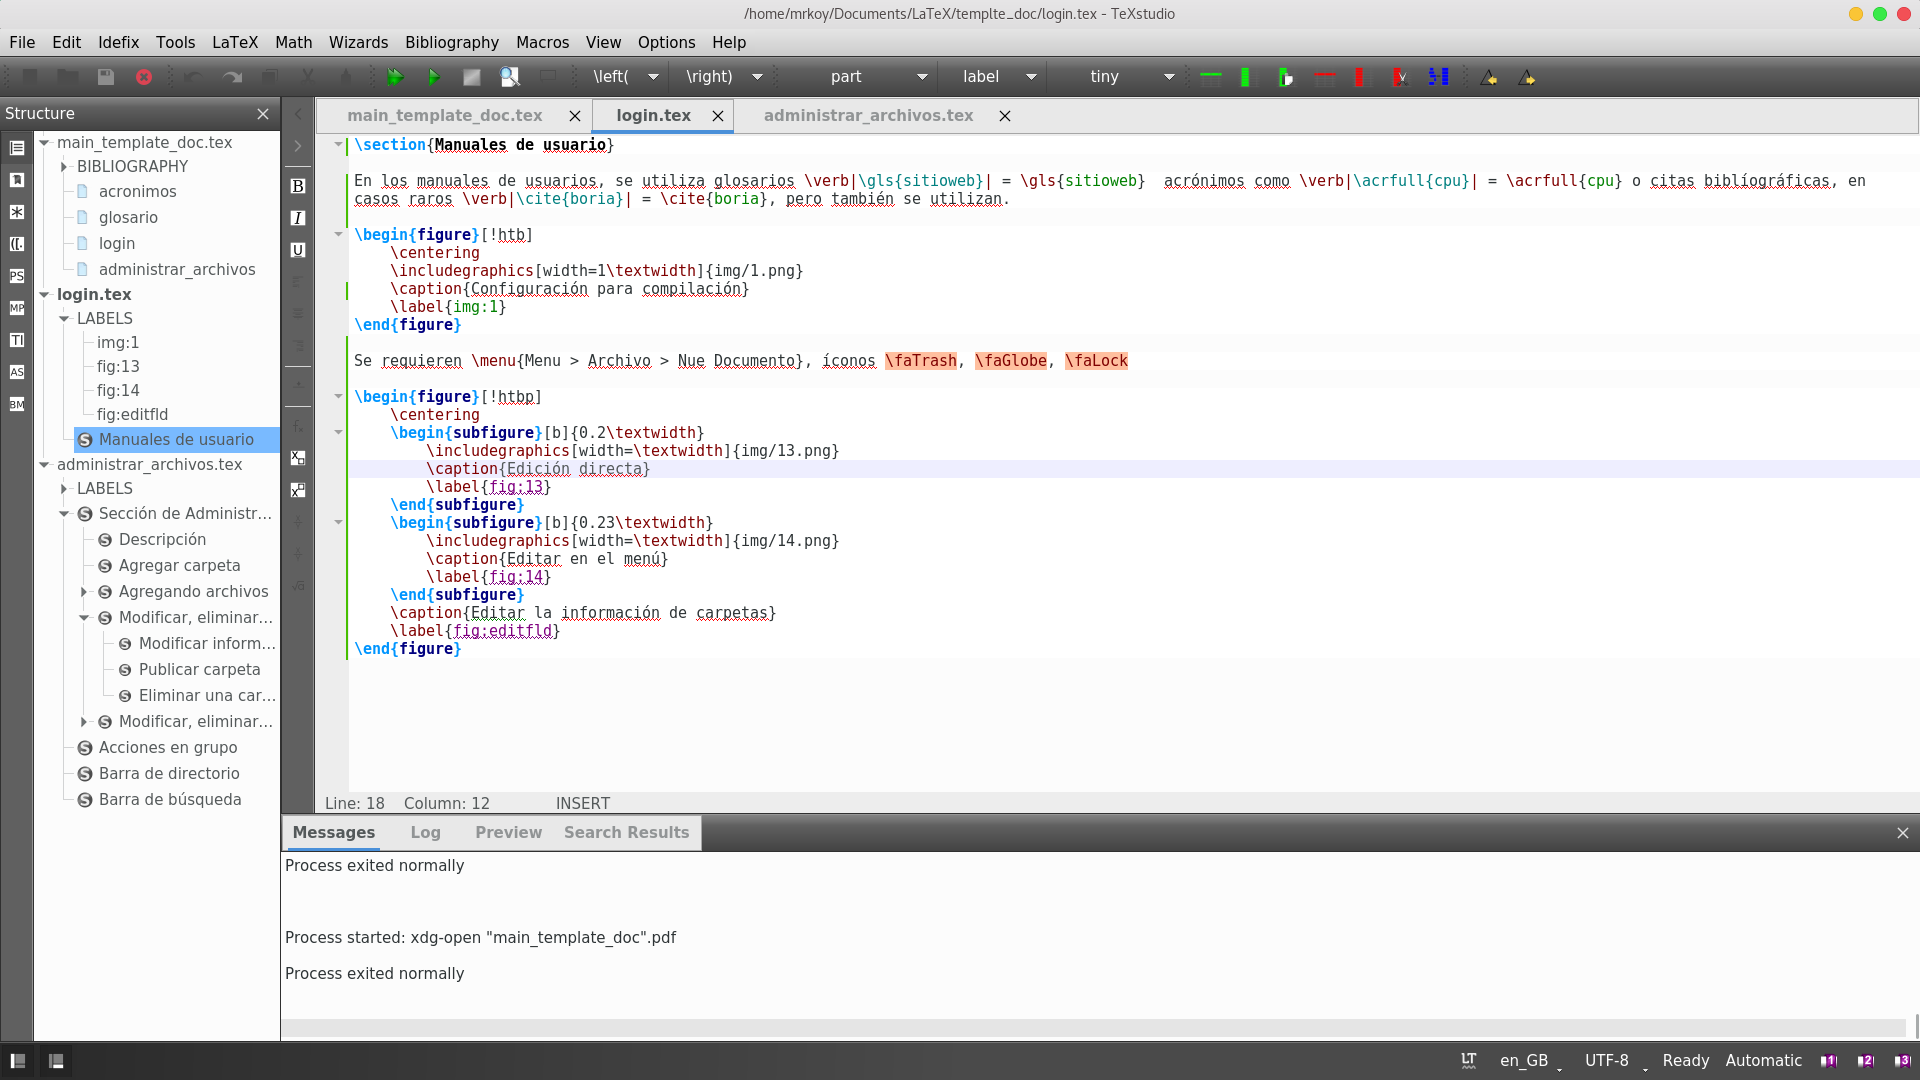
\includegraphics[width=1\textwidth]{img/3.png}
	\caption{TexStudio}
	\label{img:1}
\end{figure}

Se requieren \menu{Menu > Archivo > Nuevo Documento}, íconos \faTrash, \faGlobe, \faLock

\begin{figure}[!htbp]
	\centering
	\begin{subfigure}[b]{0.41\textwidth}
		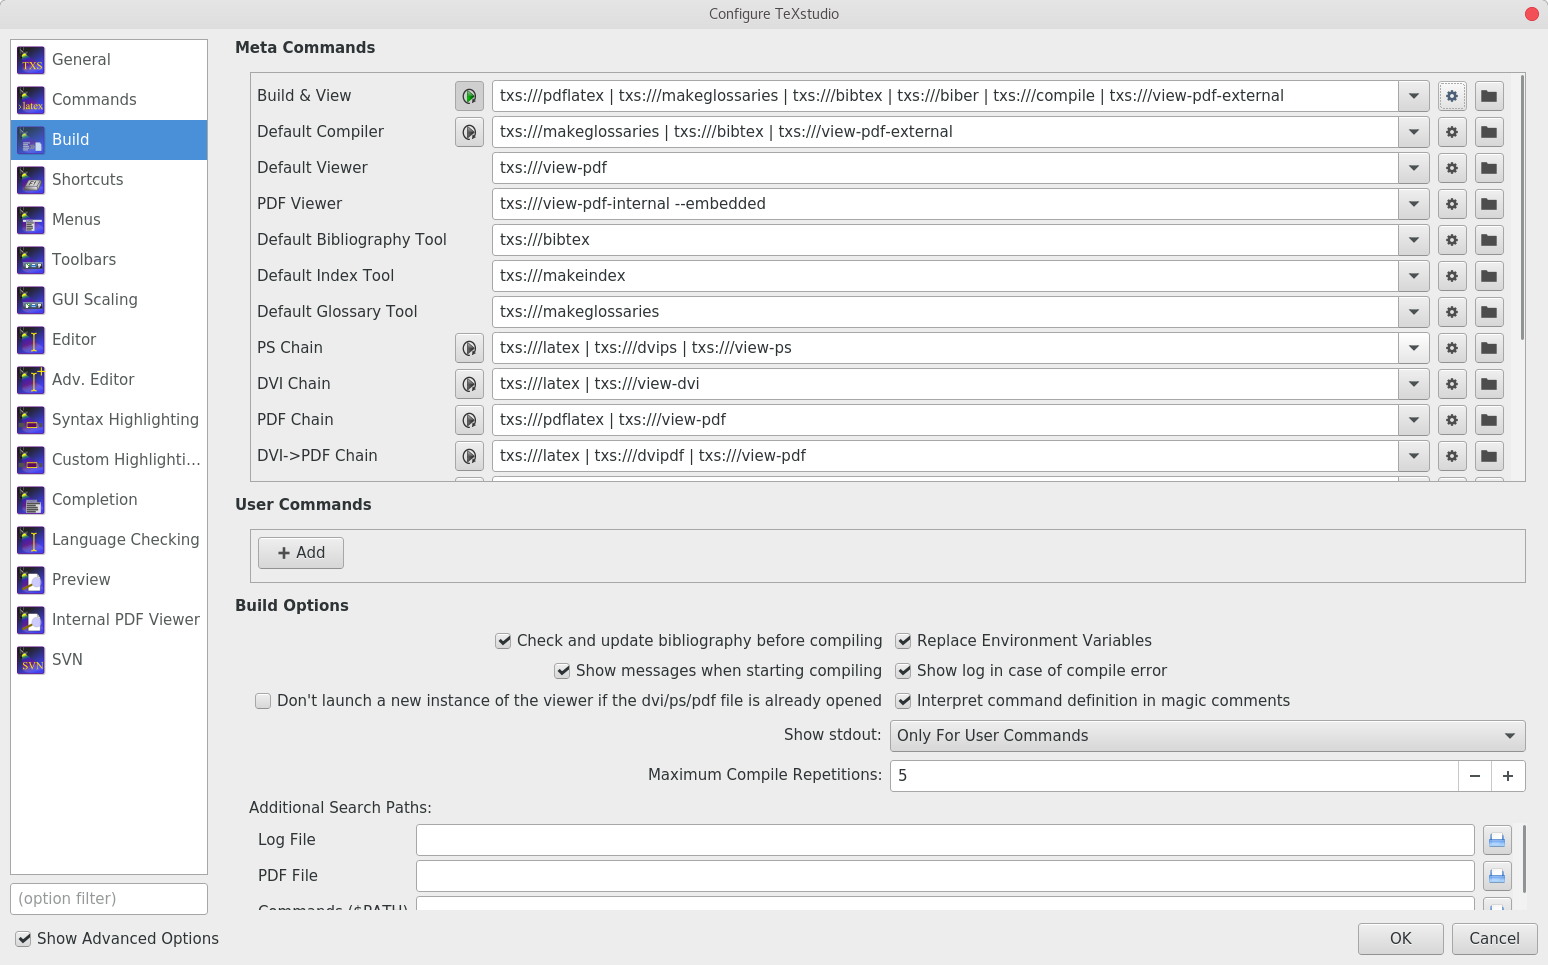
\includegraphics[width=\textwidth]{img/1.png}
		\caption{Configuración}
		\label{fig:2}
	\end{subfigure}
	\begin{subfigure}[b]{0.52\textwidth}
		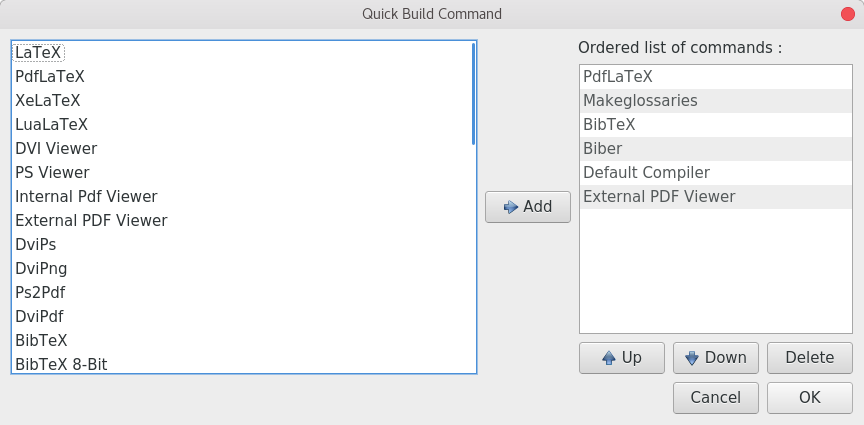
\includegraphics[width=\textwidth]{img/2.png}
		\caption{Orden de compilación}
		\label{fig:3}
	\end{subfigure}
	\caption{Configuración para compilación}
	\label{fig:compile}
\end{figure}

\section{Códigos}

Sin duda alguna habrá fragmentos de código:

\begin{mdframed}[linecolor=black, topline=false, bottomline=false, leftline=false, rightline=false, userdefinedwidth=\textwidth]
\captionof{lstlisting}{Fragmentos de código}
\label{cod:gauss}
\vspace{-0.3cm} %separción entre el caption y el código
\begin{minted}[mathescape, breaklines, frame=single, tabsize=4, gobble=0, linenos, numbersep=5pt,]{c}
////////////////////////////////////////////////
// Función de membresía Guassiana 
//$f(x)=e^{-\alpha \frac{x - c}{\delta}^2}$
////////////////////////////////////////////////

double gaussiana(double centro, double ancho, double x){
	double ux=0;
	ux=pow(2.718281828, ( -.5* pow(((x-centro) / ancho), 2)));
	return ux;
}
\end{minted}
\end{mdframed}

\section{Imágenes}
Una de las principales características de los manuales, es que llevan muchas imágenes, muchas [...]

\begin{figure}[!htb]
	\centering
	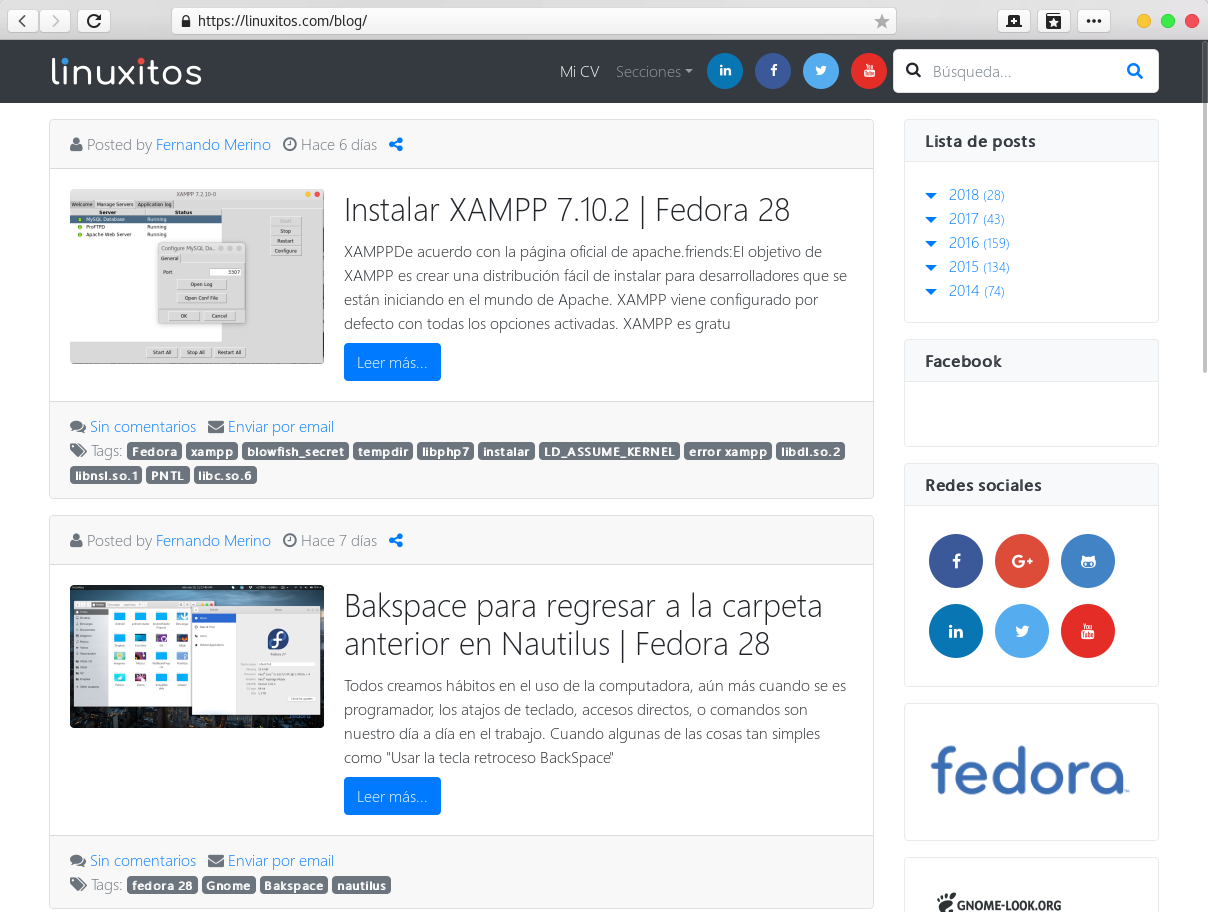
\includegraphics[width=1\textwidth]{img/4.png}
	\caption{\url{https://linuxitos.com/blog/}}
	\label{img:4}
\end{figure}

\section{Terminal}
Si es un manual sobre linux, entonces, habrá fragmentos de comandos:

\begin{myminted}{Terminal}
	sudo dnf -y install evince gedit zip file-roller xz lzma
\end{myminted}




